\documentclass[11pt, a4paper]{article}
\usepackage[czech]{babel}
\usepackage[utf8]{inputenc}
\usepackage{a4wide,color,graphicx,listings}

\title{\textbf{Jabber dungeon}}
\author{Michal Staruch\\
		Ondřej Hlavatý\\
		Petr Mánek}
\date{}

\def\class#1{\emph{#1}}
\def\jid{\texttt{dungeon@eideo.cz}}
\newenvironment{example}%
{\smallskip\noindent\ignorespaces\obeylines\tt}%
{\smallskip\par\noindent
\ignorespacesafterend}

\def\user{\textcolor{blue}{$<$user$>$ }}
\def\dung{\textcolor{red}{$<$dungeon$>$ }}
\lstset{
  keepspaces=true,
  basicstyle=\footnotesize,
  language=C++,
  tabsize=4,
  showspaces=false,
  showstringspaces=false
}

\begin{document}

\maketitle

\section{Zadání}

Projekt byl zadán jako zápočtový program na MFF UK. Cílem bylo vytvořit herní systém textové adventury, kterou bude možno hrát přes komunikační síť Jabber. Samotná adventura by měla být rozumně ovladatelná textovými příkazy a komunikovat s uživatelem přirozeným jazykem - v angličtině. Herní svět je společný pro všechny hráče, kteří se v něm pohybují nezávisle.

Jako jazyk implementace byl zvolen \texttt{C++}. Součet schopností programovat v týmu byl pro tento jazyk největší, a zároveň je vhodný pro objektový návrh.

\section{Základní návrh}

Srdcem celé hry jsou objekty \class{GameManager} a \class{ActionQueue}. Většinu informací přenáší objekty \class{ActionDescriptor} (AD). Komunikace s uživatelem probíhá skrz \class{Driver}.

Nejprve, jak vypadá životní cyklus \class{ActionDescriptoru}.
\begin{figure}[htp]
\centering
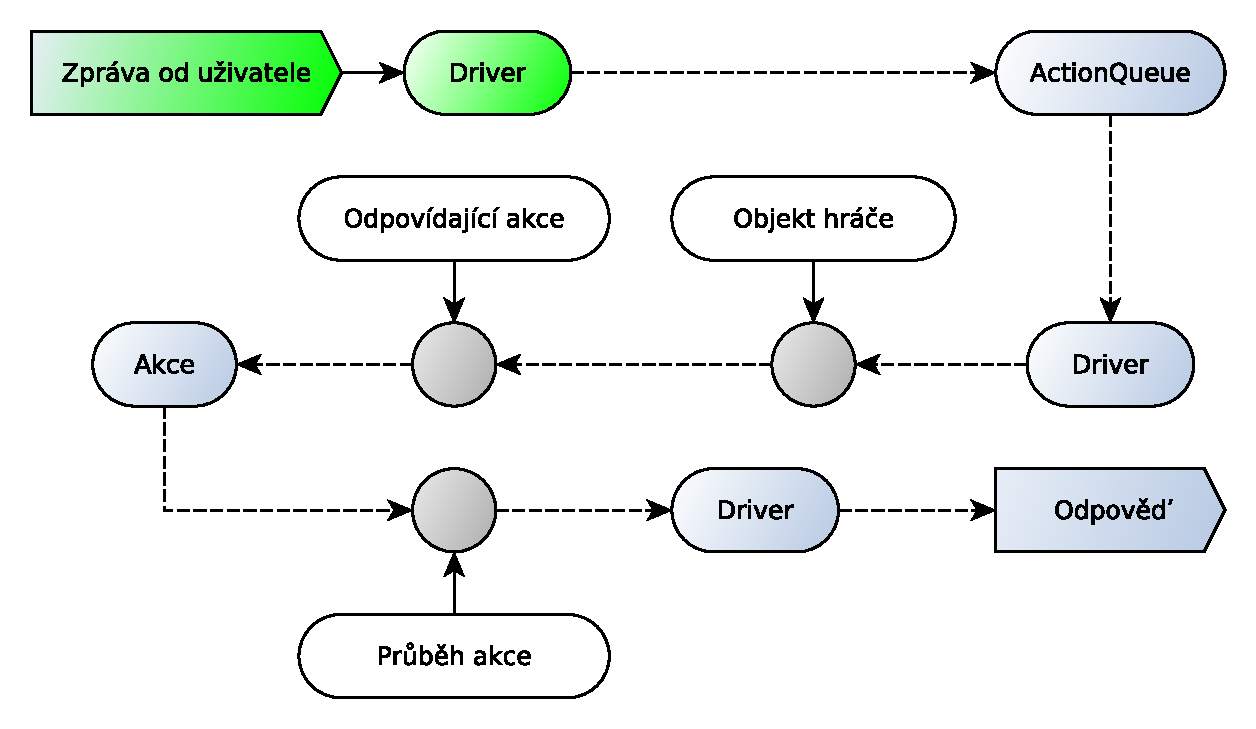
\includegraphics[scale=0.6]{AD-lifecycle.pdf}
\caption{Životní cyklus \class{AD}}
\label{ad-lifecycle}
\end{figure}

Každý běžící \class{Driver} má své vlastní vlákno (na obrázku zeleně), odlišné od hlavního herního vlákna (modře). V okamžiku přijetí zprávy vytvoří driver objekt AD nebo jeho potomka. Uloží si do něj všechny potřebné informace pro další zpracování (odesílatele, text zprávy atp.) a  zařadí jej do fronty v ActionQueue. Ta pak ve svém vlákně přiděluje čas na zpracování akce postupně a zajišťuje tím atomicitu operací \uv{zadarmo}. Když na tuto akci dojde řada, tak se teprve zjišťuje Driver co vlastně má provést. Jako první sváže akci s herním objektem uživatele - v tomto vlákně již má přístup k databázi. Poté z věcí v okolí sežene seznam proveditelných akcí a zjistí, která odpovídá vstupnímu textu. Jakmile je akce svázána, předá se řízení dané akci. Ta provede změny v herním světě a vloží do AD informace potřebné k sestavení odpovědi.

Stručně pár dalších důležitých tříd v návrhu:

\paragraph{GameManager (GM)} zprostředkovává samotný přístup k herním objektům a světu. Izoluje herní mechanismy od úložiště informací, zpřístupňuje některé zkratky.

\paragraph{ObjectPointer (OP)} Během načítání herních objektů se může stát, že GM odstraní z paměti jiný načtený objekt z důvodu úspory paměti. OP umožňuje při přístupu objekt nechat znovu načíst.

\paragraph{Driver} Implementovány jsou aktuálně \class{TextDriver}, obsluhující zprávy textového charakteru, a jeho potomci \class{ConsoleDriver} a \class{JabberDriver}. Jeden umožňuje ovládat postavu ze standartního vstupu a zprávy vypisovat na standartní výstup, druhý se přihlašuje jako jabber klient s adresou \jid a komunikuje pomocí XMPP.

\paragraph{Action} Její potomci reprezentují proveditelnou akci. Obsahuje zejména metodu \texttt{match}, která porovnává vstup od uživatele s očekávaným vzorem (regulárním výrazem) a metodu \texttt{commit}, která spustí provedení akce.

\paragraph{ActionDescriptor} Třída reprezentující komunikaci s jedním konkrétním uživatelem a provedení jedné, nebo i více akcí. Pamatuje si přijatou zprávu od uživatele a uživatele, který ji odeslal a ukládá si všechny odpovědi, které se mají odeslat zpět k uživateli.

\paragraph{Output} Dodat...

\paragraph{Base} Každý objekt ve hře implementuje toto rozhraní. Obsahuje metody pro zjišťování informací o objektu, persistenci vlastností a udržování relací.

\section{Reprezentace herního světa}

Každý objekt ve hře má svůj unikátní textový identifikátor a je instancí třídy implementující rozhraní Base. Téměř každý objekt také implementuje rozhraní \class{IDescriptable}, které poskytuje objektu název a rozsáhlejší popis. 

Objekty mezi sebou uchovávají relace, což jsou orientované hrany s daným typem. Mezi dvěma objekty může existovat pouze jedna relace od každého typu a směru.

\subsection{Persistence}

Jednotlivé vlastnosti objektů i relace jsou uchovávány v databázi. Relace jsou uložitelné jednoduše, na vlastnosti objektů má každý potomek IObjectu metodu \texttt{registerProperties}. V ní ohlásí, jaké vlastnosti má. Tyto data využije objekt \class{Archiver} a serializuje data do binárního streamu. Ten se pak může do databáze uložit. Stejnou metodou se pak data do objektu dají načíst zpět -- obrátí se směr Archiveru, a ten místo čtení hodnoty nastaví. Neví přitom nic o tom, jaké hodnoty ukládá, stačí mu k tomu typ.

To ale není jediné využití této metody. Dá se ji podstrčit libovolný objekt implementující \class{IPropertyStorage}, například administrátorský nástroj \class{PropertyEditor}, který je využije k pohodlné úpravě všech vlastností objektu přes libovolné herní rozhraní.

\subsection{Uchovávání v paměti}

Herní svět může být snadno docela veliký, proto jej nikdy nechceme načítat do paměti celý. Všechny herní objekty se proto načítají na vyžádání v době potřeby, kde to jde tak se používá pouze id objektu, předávané pomocí OP. Pro uchovávání již načtených objektů používáme Splay strom, protože umožňuje rychle přistupovat k objektům, které se používají hodně.

V současné chvíli to není implementováno, ale je možné tento strom upravit tak, aby objekty v určité hloubce (tedy dlouho nepoužité) zahazoval, a tím uvolnil paměť.

Z databáze načítá objekty \class{ObjectLoader}, ke čtení vlastností se využívá Archiveru. \class{DatabaseHandler} uzavírá práci s databází, používáme SQLite.

\section{Herní objekty a akce}

Jak už bylo řečeno, všechny objekty dědí Base a zpravidla také IDescriptable. Základní vlastností herního objektu je schopnost zjistit akce dostupné na tomto objektu. Tak je dosaženo maximální flexibility světa. Není třeba mít na jednom místě seznam všeho co lze kdykoli provést, a v různém kontextu se mohou stejné zprávy vyhodnotit různě. 

Při zpracovávání akce se v jednu chvíli zjistí akce na všech objektech v okolí uživatele, a postupně se na nich spouští metoda \texttt{match}. Jakmile se první akce k příkazu přihlásí, je provedena a na ostatní se již nedostane.

Dalšími obecnými typy objektů jsou:

\paragraph{Alive, Human} Reprezentují žívé objekty a uživatele. Každý živý objekt má své umístění a vlastnosti týkající se boje (tzn. životy, útočné a obranné číslo.) Dostupné akce na těchto objektech jsou ty které se týkají pouze daného uživatele. Tj. zjišťující aktuální stav, různé nápovědy, přejmenování atp.

\paragraph{Creature} Reprezentují všechny objekty, na které se dá útočit, tedy všechna monstra a živočichy. Akce na tento objekt je zejména attack.

\paragraph{Item} Cokoli, co jde uchopit. Objekt samotný nemá akce, ale má vlastnosti \texttt{size} a \texttt{weight}, udávající velikost a váhu objektu.

\paragraph{Wearable} Potomek třídy \class{Item}, co jde použít jako část oděvu. Tento objekt používají zbraně a různé typy brnění. Umožňuje objektům měnit bojové vlastnosti postav.

\paragraph{Inventory} Potomek \class{Wearable}, přidává navíc akci drop a umožňuje v sobě ukládat předměty.

\paragraph{Location} Reprezentuje lokaci, ve které se ostatní objekty nacházejí. Tyto lokace jsou buď místnosti, které jsou s ostatními místnostmi spojeny dveřmi, nebo truhly, které obsahují předměty. Akce na lokaci jsou zejména průzkum a sebrat věc ležící v lokaci.

\paragraph{Door} Jedno nebo obousměrný teleportační tunel mezi dvěma lokacemi. Akcí na tomto objektu je průchod skrz. Může mít také speciální zámek, který lze odemknout pouze přiřazeným klíčem.

\paragraph{Crafter} Speciální objekt, který je používán pro tvorbu věcí. Udržuje v sobě objekty \class{Recipe}, které říkají, jaké věci umí \class{Crafter} vyrobit. Ve hře se vyskytuje například jako kovadlina.

\paragraph{Resource} Potomek třídy \class{Item}, reprezentuje věci, které se seskupují, tedy například peníze, nebo materiály pro \class{Crafter}. Má na sobě metody \texttt{split} a \texttt{join}, které umožňují objektům vyjadřující stejnou \class{Resource} se buď rozdělit na dva podobjekty, nebo spojit do jednoho objektu.

\paragraph{Interactive} Jednoduchá obálka pro vytváření herních objektů, jako jsou cedule, nebo někdo, s kým si může hráč promluvit. Přidává pouze k zkratky k zajištění tohoto chování, více viz sekce \texttt{Behavior}

\paragraph{Spell} Umožňuje používat kouzla. Každý hráč se kouzlo naučí přečtením speciálního svitku. Mezi kouzla se dají například zařadit léčivá, nebo teleportovací kouzla.

\paragraph{ThorsHammer} Speciální objekt, který vlastní administrátoři. Pomocí tohoto objektu se dá zasahovat do herního světa nebo i běhu programu. Administrátorovi umožňuje měnit objekty pomocí vnořené třídy \class{PropertyEditor}, upravovat si počet surovin, nebo například vyžádat ukončení serveru.

\subsection{Parametrizované akce}

Velmi častým požadavkem je, aby akce měla nějaký parametr. Například když v místnosti leží tři lektvary, je potřeba určit který z nich se má akcí vypít. Tento problém důstojně řeší \class{MultiTargetAction} (MTA). Objekt vytvoří instanci MTA, a do seznamu cílů přidá sám sebe nebo i jiné objekty, na které lze akci zacílit. Při přidávání do seznamu se podle identifikátoru zjistí, že stejný druh akce již v seznamu je, a seznamy cílů se spojí v jeden. Akce si potom při spuštění vybere ze seznamu ten objekt, který nejlépe odpovídá zadanému textu.

Zároveň, pokud je v místnosti pouze jeden lektvar, pak spuštění akce vypije právě ten jeden lektvar i bez bližšího určení.

Při výběru objektů se porovnává editační vzdálenost (Damerau-Levenshteinova) slov z názvu objektu od slov ze zadaného textu. Při počítání vzdálenosti je změna znaku pocítána jako větší úprava, než přidání či odebrání. Počítají se pouze dostatečně podobná slova ve správném pořadí. Proto přidání neurčujících slov (členů, zájmen) neovlivní volbu, a naopak nespecifikování částí názvu (bližší popisy) nemusí nutně znamenat chybu ve výběru. Pokud se nedokáže mechanismus rozhodnout, který objekt vybrat, dá uživateli na výběr.

Tento mechanismus je silně spojen s objektem \class{MTATrap}, který zajišťuje přerušení akce a umožňuje dát uživateli na výběr, co se má provést bez toho, aby byly ztraceny informace o pasti. Tento objekt navíc umí rozpoznat speciální klíčová slova, jako jsou například \textit{it}, \textit{any}, \textit{none} apod.

\section{Další (nejen) herní mechanismy}

\subsection{Skupinový popis}

Aby hraní působilo přirozeněji, popisovatelné objekty se umí sdružit podle typu a vypsat jednotný popis za všechny. Funkcionalitu zajišťuje třída \class{ObjectGroup}. Výpis pak může vypadat třeba takto:

\begin{example}
\dung You see Piece of wood and Stone. There lies Red potion, Green
potion and Blue potion. 
\end{example}

\subsection{Dialogy}
\label{dialogs}
Zpočátku vypadal hra striktně podle režimu příkaz -- odpověď, a hra připomínala spíše příkazový řádek\footnote{Z čehož vznikly aliasy pro akce, např. \texttt{cd} pro průchod dveřmi :)}. Toto schéma rozbíjí mechanismus dialogu:

\begin{example}
\user rename myself
\dung Well then, what do you want your new name to be?
\user New name
\dung OK. You shall now be called New name. I'm just curious, why did 
you change your name?
\user Because I wanted to show, how dialogs work.
\dung Interesting. Now, back to the dungeon!
\end{example}

\subsection{Boj}
\label{combat}
Systém boje vznikl krátce po vzniku dialogů a hojně jich využívá. Každá instance třídy \class{Creature} přidá akci \texttt{attack}, která inicializuje boj. Po zavolání akce \texttt{attack} se pustí obslužná metoda, která vždy provede požadovanou akci a v dialogu se zeptá uživatele, co dělat dále. Pokud hráč dosáhne 0 životů, zemře, pokud dosáhne 0 životů \class{Creature}, nastane smrt příšery.

\subsection{Smrt}

Smrt nastane, pokud životy hráče nebo nepřátel dosáhnou nuly. Metoda \texttt{changeHp}, která se stará o změnu počtu životů automaticky zavolá obslužnou proceduru \texttt{die}. V případě třídy \class{Human} procedura změní stav hráče na mrtvého, zakáže mu většinu akcí kromě některých výjimek a znemožní mu hrát po stanovený interval. Po uplynutí toho intervalu se může hráč akcí \texttt{respawn} oživit, při oživení je přemístěn do poslední místnostni s flagem \texttt{respawnable}, kterou hráč navštívil. V případě třídy \class{Creature} je na zem puštěna odměna za zabití (pokud nějaká je) a instanci se naplánuje automatický respawn, který je kontrolován (a popřípadě proveden) při zjišťování akcí.

\subsection{Pasti}

Pasti jsou velmi důležitá součást naší hry. Umožňují nám měnit svět v reakci na události a mít svět dynamičtější. Jednotlivé pasti jsou potomky třídy \class{Trap}. Ta definuje 2 metody:
\begin{itemize}
\item metodu \texttt{trigger}, která je zavolána pokaždé, když se vyvolá akce, na kterou je past napojena. V této metodě se rozhodne, jestli se past má pustit a něco udělat, nebo nechat svět plynout dále.
\item metodu \texttt{exceptionTrigger}, ta reaguje na výjimky \class{TrapException}. Tato výjimka je vyhozena v metodě \texttt{trigger} a její smysl je měnit probíhající akce. Tato metoda může akci zrušit, nebo ji změnit (například past \class{AttackTrap}, která zahájí boj při vstupu do místnosti.)
\end{itemize}
V současné době máme ve hře několik pastí, například \class{HealingTrap} (past, která léčí jednoho uživatele, nebo všechny v místnosti), \class{AttackTrap} (nechá něco zaútočit na uživatele), \class{DoorLock} (past, která se chová jako zámek na dveřích), nebo \class{ItemRespawner} (past, která umožňuje věcem se znovu objevit po určitém intervalu.)

\subsection{Behavior}

Potomci třídy \class{Behavior} přidávají jednoduchý způsob, jak zajistit modulární chování herních objektů. Přidáním speciální relace na původním objektu se objekt spáruje s objektem chování, který přidává novou akci na objektu. Tímto můžeme pouze přidáním jednoduché relace například přidat objektu nápis, který lze přečíst bez toho, abychom museli mít vytvořený speciálního potomka objektu, který by přidával akci čtení.

\section{Programová část}

V této kapitole bychom chtěli vypíchnout některé části kódu, které se nám líbí, jsou zajímavé, nebo se k nim váže nějaká příhoda.

\subsection{Logování}

Podstatnou částí systému, na kterou jsme patřičně hrdí, je logovací mechanismus. Jeho srdcem je třída \class{Logger}, se kterou aplikace komunikuje během hry v singletonovém režimu použitím několika šikovných maker.

\begin{lstlisting}
	LOGS(Fatal) << "Error saving object "
	                      << id << ", error code " << err << LOGF;
	                      
    LOG << ... // default is Severity::Info
    
    LOGH("Database cleanup") // creates headline for the next section
\end{lstlisting} 

\noindent
Díky přetížení operátoru \texttt{<<} můžeme logovat téměř jakýkoliv druh obsahu. Protože každý záznam uvádí kromě zprávy i důležitost, chyby nezapadnou mezi běžnými záznamy.

Všechny záznamy z logu jsou přesměrovány skrz buffery do výstupů – podtříd \texttt{std::ostream}. Tento objektový přístup je velmi praktický, protože nám umožňuje postavit výstupní soubory na stejnou úroveň jako standardní výstup aplikace. Navíc můžeme pro každý výstup nastavit minimální důležitost, od které události zaznamenává. V současném stavu se log ukládá takto:

\begin{itemize}
\item na \texttt{stdout} proudí zprávy s důležitostí $>=$ \texttt{Severity::Info}.
\item do souboru \texttt{YYYY-MM-DD-stdout.log} se kopíruje \texttt{stdout}
\item do souboru \texttt{YYYY-MM-DD-verbose.log} proudí úplně všechny zprávy
\item do souboru \texttt{YYYY-MM-DD-warnings.log} proudí zprávy s důležitostí $>=$ \texttt{Severity::Warning}
\item do souboru \texttt{YYYY-MM-DD-debug.log} proudí debugovací zprávy. Z důvodu velkého množství takových zpráv je tento výpis vypnutý a je možné ho zapnout pomocí parametru \texttt{-d}
\end{itemize}

\noindent
\textit{(soubory jsou opatřeny datem zapnutí aplikace a zapisuje se do nich režimem append)}

\noindent
V případě potřeby můžeme kdykoliv toto nastavení změnit i za běhu aplikace. Typickým příkladem této operace je parametr \texttt{-v}, se kterým se na obrazovku vypisují také záznamy úrovně \texttt{Severity::Verbose}. Této změny dosáhneme jedním řádkem kódu:

\begin{lstlisting}
    Logger::getInstance().setMinSeverity(cout, Logger::Severity::Verbose);
\end{lstlisting}

\noindent
Logování je samozřejmě thread-safe, takže se nemůže stát, že by některá vlákna aplikace (například \class{JabberDriver}) mohly začít zapisovat uprostřed zapisování jiného záznamu.

\subsection{Výběr náhodné zprávy}

Pro ozvláštnění komunikace je dobré nemít všude stejné statické texty, ale výpis trochu měnit.

\begin{example}
\user something
\dung One does not simply ask me to "something".
\user something
\dung I wouldn't do that if I were you. Besides, I can't do that.
\user something
\dung The day may come when I understand "something"{} but it's not 
this day.
\end{example}

\noindent Pro tento účel jsme si napsali utilitku \class{RandomString}, která se používá takto:

\begin{lstlisting}
	return RandomString::get()
		    << "What do you mean \"" + input + "\"?" << endr
		    << "One does not simply ask me to \"" + input + "\"." << endr
		    ...
			<< "This is not the thing you are trying to do." << endr;
\end{lstlisting}

\noindent Třída využívá přetížení operátoru \texttt{<<} a přetypovaní na string.

\subsection{Spojování částí vět}

Protože hra s uživatelem komunikuje textově, brzy jsme přišli na to, že potřebujeme elegantní způsob, jak skládat jednoduše části vět dohromady. K tomu jsme vytvořili třídu \class{SentenceJoiner}. Instanci této třídy předáme jednotlivé části vět (slova, nebo slovní spojení) a šablonu výstupní věty. \class{SentenceJoiner} za nás poté spojí části dohromady pomocí správných spojek a vrátí nám správně zformátovanou větu.

\noindent Největší sílu má tento mechanismus v kombinaci s náhodným vybíráním zpráv.

\subsection{InstanceOf}

Potřeba použití nečeho takového signalizuje chybu v návrhu, ale pokud chceme mít obecný mechanismus práce s objekty, je občas potřeba o obecném \texttt{Base*} zjistit něco více. Proto se hodí tento operátor. Použití:

\begin{lstlisting}
	Alive* A;
	A->instanceOf(Backpack); // true / false
\end{lstlisting}

\noindent Celá věc funguje trochu magicky, ale hlavně rychle. Pomocí preprocesorových maker se v každém objektu vytvoří virtuální inline funkce \texttt{className} a \texttt{isInstanceOf}. ClassName vrací konstantní řetězec obsahující název třídy -- ten se používá například pro serializaci do databáze. Pro použití s instanceOf se ale počítá jen s ukazatelem na tento řetězec. Pomocí dalších maker se ukázka přepíše takto (s využitím konstanty):

\begin{lstlisting}
	A->isInstanceOf(Backpack::BackpackClassName); // true / false
\end{lstlisting}

\noindent A protože je funkce inline, kompilátor ukázku přepíše například takto:

\begin{lstlisting}
	Alive::AliveClassName == Backpack::BackpackClassName 
		|| IDescriptable::IDescriptableClassName == Backpack::BackpackClassName 
		|| Base::BaseClassName == Backpack::BackpackClassName;
\end{lstlisting}

\noindent Celý operátor tedy pouze projde hiearchii volané třídy a porovná ukazatele na tento konstantní řetězec.

\subsection{Dialogy}

O tom jak vypadají dialogy v praxi bylo již psáno v části \ref{dialogs}. Jak se ale dialogy používají? Příkladem je celý kód akce na přejmenování uživatele:

\begin{lstlisting}
	*ad << "Well then, what do you want your new name to be?";
	ad->waitForReply([] (ActionDescriptor *ad, string reply) {
		((Human*) ad->getAlive())->setUsername(reply)
				->save();
		*ad << "OK. You shall now be called " 
			<< ad->getAlive()->getName() << ". "
		    << "I'm just curious, why did you change your name?";
	});
	ad->waitForReply([] (ActionDescriptor *ad, string reply) {
		*ad << "Interesting. Now, back to the dungeon!";
	});
\end{lstlisting}

\noindent ActionDescriptor umožňuje zařadit do své vnitřní fronty lambda funkci, která bude reagovat na odpověď uživatele. Pokud AD nemá frontu prázdnou, musí si jej Driver někde zapamatovat a vrátit se k němu při přijetí další zprávy.

Všechny lambda funkce nemusí být vytvořeny hned, dají se vytvářet postupně. Tento zápis je však přehledný, a z kódu je hned vidět jak dialog probíhá. Zároveň je ale možno udělat dialog, který není lineární, nebo třeba není předem známý - například boj.

Dialog ale může rozbít atomicitu operací, jelikož při čekání na odpověď od uživatele mohou probíhat jiné akce, je tedy potřeba po získání odpovědi zkontrolovat stav herního světa, aby nedošlo k ilegální úpravě světa.

\subsection{Cloner}

Původní myšlenkou bylo to, že všechny objekty budeme vytvářet ručně a během hry. Postupem času se však ukázalo, že toto není nejlepší nápad a tak jsme hledali způsob, jak objekty vytvářet rychleji.

Nakonec jsme přišli s třídou \class{Cloner}, která využívá vlastnosti objektů a pomocí \class{IPropertyStorage} je schopen je přečíst. Při jejich čtení si je ukládá do své paměti. Po přečtení využije další metodu naší perzistence a tou je \texttt{createObject}, kterou vytvoří čistou kopii objektu. Poté z uloženého seznamu nahraje všechny vlastnosti nového objektu, změní mu \texttt{id} a vrátí tento objekt. Tuto kopii nazýváme \texttt{shallowCopy}.

\class{Cloner} umí vytvořit ještě \texttt{deepCopy}, která navíc zkopíruje všechny relace objektu.

Tuto třídu hojně využíváme při vytváření světa ve třídě \class{WorldCreator}, kde nejprve vytvoříme vzory všech objektů a poté už je jenom rozkopírujeme, kde je potřeba.

\subsection{Konfigurace světa}

Původně jsme měli přímo v kódu některé konstanty, kterými jsme například nastavovali název databáze, nebo dobu oživení hráče. S přibývajícím počtem těchto konstant jsme ale zjistili, že ukládat konstanty přímo do kódu je nepraktické a tak vznikly třídy \class{Config} a \class{ConfigParser}. 

Třída \class{Config} má statické metody k zjišťování nastavení, které čtou privátní proměnné jediné instance této třídy. Tím je zajištěno, že není možné hodnotu této proměnné změnit někde v kódu. 

Třída \class{ConfigParser} poté zabaluje čtení konfiguračního souboru. Při předložení souboru instanci této třídy si ho instance načte do mapy v paměti, na kterou se poté ptá \class{Config}. Některé metody této třídy nabízejí možnost předat i lambda funkci, která může dále kontrolovat přečtené hodnoty (například na rozsah, nebo nějaký výčet hodnot).

\section{Ukázky}

Rádi bychom ukázali nějaké naprosto základní ukázky komunikace s programem.
\subsection{Průzkum světa}

\begin{example}
\user hello
\dung Hi!
\user where am i
\dung You are in Base Camp. Nothing much to be found here, but get
familiar with basic commands - try to type 'help'. There is a wooden
door. You recognize Salmelu and CiTrus. You have a Leather backpack 
with you.
\user go to that wooden door
\dung You are in Equip room. Looks like noone has been there for 
a long time. There is a wooden door. You see Green potion, Blue potion 
and Red potion. 
\user drink the blue potion
\dung You've drunk Blue potion. You've healed 100 hitpoints
\user pick the red potion
\dung You've picked up Red potion.
\user explore
\dung You are in Equip room. Looks like noone has been there for 
a long time. There is a wooden door. You see Green potion lying on the 
ground. You have a Leather backpack with you. There is Red potion.
\user drop the red potion
\dung You've dropped Red potion. 
\end{example}
\subsection{Systém boje}
\begin{example}
\user explore
\dung You are in Landcastle. A nice stone castle, having a magical aura surrounding it. You feel the aura and feel much better here. If you are confused what to do, try typing 'help'. Around you are Bridge and Climb. You smell the presence of Aearsis and CiTrus.
\user go to bridge
\dung You walk over the bridge. Seems like you are in Faygrass. A vast grass field. You see Rat and Rat wandering around. You see Small spider wandering around. Around you are Muddy walkway, Bridge and Stairs.
\user attack spider
\dung You have dealt 7 damage to Small spider by your Wooden axe. Small spider caused you 10 damage by its poisoned bite. Your current hitpoints have changed to 290. Type 'attack' (a) to attack the enemy, 'check' (c) to check its status or 'run' (r) to run from the fight. 
Small spider: [*******---]     You: [**********]
\user attack
\dung Your Wooden axe have caused 7 damage to Small spider. Small spider caused you 10 damage by its poisoned bite. Your current hitpoints have changed to 280. Type 'attack' (a) to attack the enemy, 'check' (c) to check its status or 'run' (r) to run from the fight. 
Small spider: [****------]     You: [**********]
\user a
\dung Your Wooden axe have caused 6 damage to Small spider. Small spider is mortally wounded. Use 'kill ...' to finish it.
\user kill spider
\dung Small spider has dropped nothing. You have killed Small spider.
\end{example}
\subsection{Resources}
\begin{example}
\dung You are in Shadowcliff. Dark dangerous cliffs. You shouldn't leave the path you are currently on. You see Rat wandering around. There lie corpses of Small spider and Small spider. You see Pathway and Climb. You see 58 sand and 78 sand lying there. There lies 41 white powder and 31 white powder.
\user pick 58 sand
\dung You've picked up 58 sand.
\user pick 78 sand
\dung You've picked up 78 sand.
\user pick 41 white powder
\dung You've picked up 41 white powder.
\user pick 31 white powder
\dung You've picked up 31 white powder.
\user list items
\dung As your backpack, you're using Leather backpack. There are 136 sand and 72 white powder. Wooden axe is your main weapon.
\end{example}
\subsection{Výroba věcí}
\begin{example}
\user craft table
\dung Small red potion: 12 white powder and 20 sand. Tiny red potion: 4 white powder and 8 sand.
\user create small red potion
\dung You have tried to craft Small red potion but you succeeded just barely. You have acquired a Tiny red potion and put it in your backpack.
\end{example}
\subsection{Past}
\begin{example}
\user explore chest
\dung You have cut yourself accidentaly with an icicle. You have received 37 damage. There is also some Small red potion.
\user pick potion
\dung You've picked up Small red potion.
\end{example}
\subsection{String matching}
\begin{example}
\dung Seems like you are in Shadowcliff. Dark dangerous cliffs. You shouldn't leave the path you are currently on. You see Rat wandering around. There lie corpses of Small spider and Small spider. There are Pathway and Climb. There lies 75 sand. There are 31 wood and 30 wood.
\user pick wood
\dung Sorry, did you mean 31 wood or 30 wood?
\user 31
\dung You've picked up 31 wood.
\end{example}

\subsection{Sdružující akce}
\begin{example}
\user use the wooden thing
\dung Sorry, did you mean wooden door, Wooden axe or Wooden club?
\user axe
\dung You have successfully equipped Wooden axe.
\user use the wooden thing
\dung Sorry, did you mean wooden door or Wooden club?
\user door
\dung You've gone through that door...
\end{example}
\end{document}
